\documentclass[a4paper,twoside, openright,12pt]{report}
\usepackage{psfrag,amsbsy,graphics,float}
\usepackage{graphicx, color} %Deleted [dvips] in front of {graphicx, color} for usage also with PDFLaTex
\usepackage[latin1]{inputenc}
\usepackage{verbatim}
\usepackage{tcolorbox}

% based on the LSR Student Template, last change: 2014-06-05

%_______Kopf- und Fußzeile_______________________________________________________
\usepackage{fancyhdr}
\pagestyle{fancy}
%um Kopf- und Fußzeile bei chapter-Seiten zu reaktivieren
\newcommand{\helv}{%
   \fontfamily{phv}\fontseries{a}\fontsize{9}{11}\selectfont}
\fancypagestyle{plain}{
	\fancyfoot{}% keine Fußzeile
	\fancyhead[RE]{\helv\leftmark}% Rechts auf geraden Seiten=innen; in \leftmark stehen \chapters
	\fancyhead[LO]{\helv\rightmark}% Links auf ungeraden Seiten=außen;in \rightmark stehen \sections
	\fancyhead[RO,LE]{\thepage}}%Rechts auf ungeraden und links auf geraden Seiten
%Kopf- und Fußzeile für alle anderen Seiten
\fancyfoot{}
\fancyhead[RE]{\helv\leftmark}
\fancyhead[LO]{\helv\rightmark}%alt:\fancyhead[LO]{\itshape\rightmark}
\fancyhead[RO,LE]{\thepage}
%________________________________________________________________________________


%_Definieren der Ränder und Längen__________
\setlength{\textwidth}{15cm}
\setlength{\textheight}{22cm}
\setlength{\evensidemargin}{-2mm}
\setlength{\oddsidemargin}{11mm}
\setlength{\headwidth}{15cm}
\setlength{\topmargin}{10mm}
\setlength{\parindent}{0pt} % Kein Einrücken beim Absatz!!
%___________________________________________

%_Hyperref for CC Url__________
\usepackage{hyperref}
%___________________________________________

%_______Title Page__________________________________________
\begin{document}
\pagestyle{empty}
\enlargethispage{4.5cm} %Damit das Titelbild weit genug unten ist!
\begin{center}
\phantom{u}
\vspace{0.5cm}
\Huge{\sc Real-time robot arm control using motor imaginary movements decoded from EEG
	signals}\\
\vspace{1.5cm}
		\large{
			RESEARCH PRACTICE\\%i.e. DIPLOMA THESIS, BACHELOR THESIS, ADVANCED SEMINAR,
			%Intermediate Report\\
			\vspace{0.4cm}
			submitted by\\
			Juri Fedjaev\\
			% if this is a diploma/bachelor/master thesis include the following:
			%\vspace{0.5cm}
			%born on: DD.MM.YYYY\\
			%\vspace{0.5cm}
			%Streetname XX \\
			%Zipcode City \\
			%Tel.: xxx\,xxxxxxxx \\
			\vspace{1.5cm}
			NEUROSCIENTIFIC SYSTEM THEORY\\
			Technische Universit\"at M\"unchen\\
			\vspace{0.3cm}
			Prof. Dr J\"org Conradt\\
		}
\end{center}
\vspace{5.5cm}
\begin{tabular}{ll}
Supervisor: &Dipl.-Ing. Zied Tayed \\
% add the start and intermediate report dates for DA/BA/MA thesis
%Start: & xx.xx.201x  \\
%Intermediate Report: &  xx.xx.201x  \\
Final Submission: &  22.05.2017 \\
\end{tabular}
%____________________________________________________________

\newpage	
\cleardoublepage



\phantom{u}
\phantom{1}\vspace{6cm}
\begin{center}
In your final hardback copy, replace this page with the signed exercise sheet.
\end{center}

\newpage


%_______Abstract_____________________________________________
\topmargin5mm
\textheight220mm
\pagenumbering{arabic}
\phantom{u}
\begin{abstract}
  A short (1--3 paragraphs) summary of the work. Should state the problem, major assumptions, basic idea of solution, results. Avoid non--standard terms and acronyms. The abstract must be able to be read completely on its own, detached from any other work (e.g., in collections of paper abstracts). Don't use references in an abstract.
\end{abstract}
%____________________________________________________________

\newpage

%_______Widmung_______________________________________________
\phantom{u}
\phantom{1}\vspace{6cm}
\begin{center}
%Hier die Widmung oder leer lassen
\end{center}
%_____________________________________________________________



\pagestyle{fancy}

%_________Inhaltsverzeichnis__________________________
\tableofcontents	
%_____________________________________________________32


%_________Einleitung__________________________________
\chapter{Introduction}
People with severe neuromuscular disorders, such as late-stage amyotrophic sclerosis (ALS) and those paralyzed from higher level spinal cord injury are unable to actuate any of their muscles. Communication with the outside world is therefore problematic for the suffering people. Cognitive and sensory body functions, however, are often only minimally affected. Therefore, an electroencephalogram (EEG)-based communication which does not require any neuromuscular control is considered to be particularly helpful to enhance the disabled's quality of life by increasing their independence \cite{birbaumer2006brain}.\\\\
Besides EEG, there are other techniques for monitoring brain activity, such as functional magnetic resonance imaging (fMRI), magnetoencephalography (MEG), positron emission tomography (PET) or single photon emission computer computer tomography (SPECT). The advantages of those methods are a better accuracy and better spatial resolution compared to EEG. However, due to their large size, heavy weight and high price, they are not as suitable for BCI applications as EEG. Furthermore, EEG offers a better temporal resolution, portability and relatively low cost. Recently, low-cost consumer devices came on the market (e.g. EMOTIV EPOC+), which will further push the advancements in the area of EEG-based BCI \cite{sivakamianalysis}. \\\\
In general, the information flow in a BCI follows the following path: signal acquisition, signal (pre)-processing, feature selection and extraction, classification (detection of distinct signal pattern), application interface (e.g. to a robot arm), and feedback (see figure~\ref{fig:bci_control_system}). 

\begin{figure}[htbp]
	\centering
	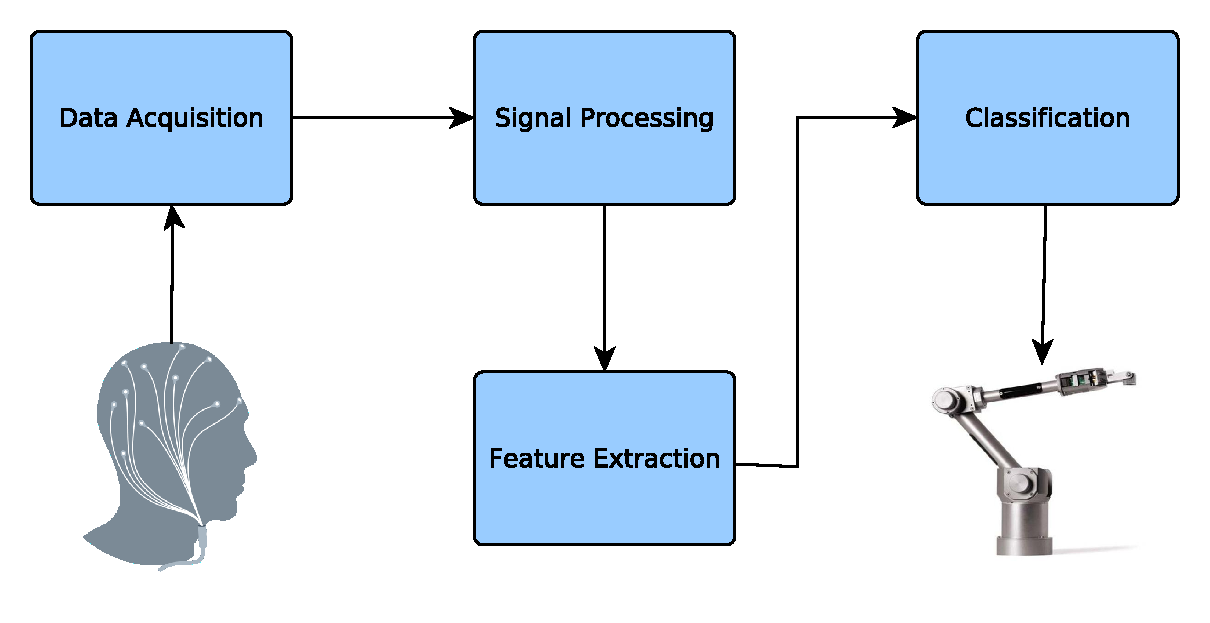
\includegraphics[width=0.8\linewidth]{./gfx/BCI_control_system.pdf}
	\caption{Information flow for a BCI system controlling a robotic arm.}
	\label{fig:bci_control_system}
\end{figure}
For the project of this research practice, the main objective is to implement algorithms similar to those described by Meng and Yong \cite{meng2016noninvasive,yong2015eeg} to discriminate and decode four motor imagery movements (left hand, right hand, both hand imaginary movement and
rest) from EEG signals. Afterwards, the classification has to be used to control a robot arm in a real-time scenario. Motor imagery (MI) is defined as the mental rehearsal or imagination of a physical movement without actually performing it physically \cite{decety1996neurophysiological}. On a neurophysiological level, similar brain regions are activated during motor execution and motor imagery, however, the performance is blocked at a corticospinal level. Studies based on fMRI showed similar activation patterns during motor imagery and actual movement execution \cite{lotze1999activation}. For operating a BCI, motor imagery has proven its capability as an efficient mental strategy. \\\\
Concerning the positioning of the EEG electrodes on the scalp, an internationally recognized method called the 10-20 EEG system is used (see fig.~\ref{fig:10-20-system} for illustration). It was developed to ensure reproducibility by standardizing the electrode positions so that one subject's studies could be compared to each other. The system is based on the relationship between the location of an electrode and the underlying area of cerebral cortex. The "10" and "20" refer to the fact that the actual distances between adjacent electrodes are either 10\% or 20\% of the total front-back or right-left distance of the skull \cite{homan1987cerebral}. Previous studies show that electrode positions C3, Cz and C4 are suitable for recording characteristic motor imagery signals, as they are directly covering part of the sensorimotor area. \\

\begin{figure}[h]
	\centering
	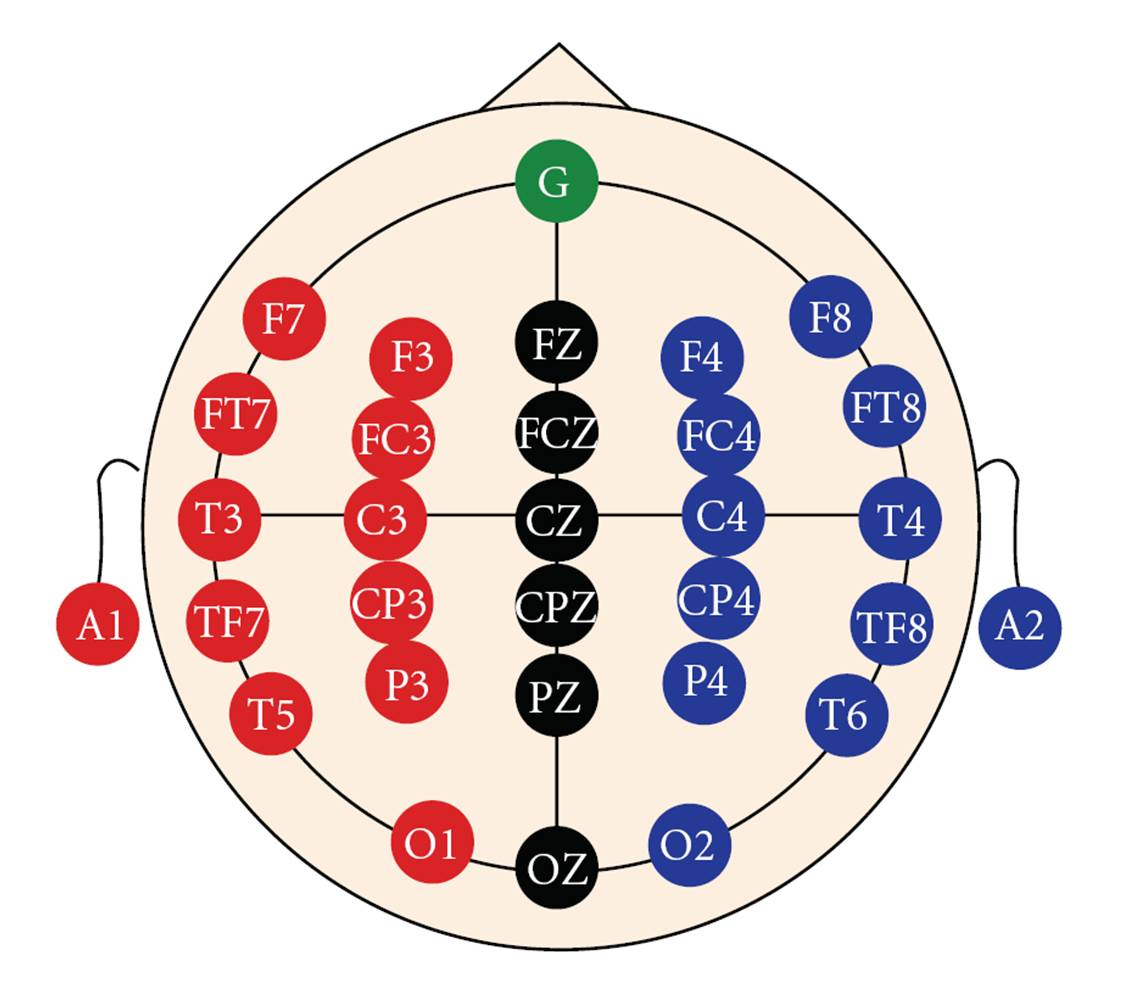
\includegraphics[width=0.5\linewidth]{./gfx/10-20.jpg}
	\caption{International standard 10-20 electrode placement system.}
	\label{fig:10-20-system}
\end{figure}



In the following, first the design and implementation of the BCI project will be discussed. Following that, the accuracies that have been reached will be presented and drawbacks of the approach and possible improvements will be discussed.




%____________________________________________________



%_____Kapitel 2_________________________________
\chapter{Solution Design and Implementation}
Figure below depicts the essential information flow for a BCI system. 




\section{Experimental Design}
In this section the design of the proposed solution will be described, i.e. the overall architecture on an abstract level. 

\begin{itemize}
	\item OpenVibe
	\item BCILAB
	\item ... 
	\item my Design
	\subitem time-constraint is present, because experimental design is a cue-based approach
\end{itemize}

Experiment design:
\begin{itemize}
	\item cue-based experiment
	\item acquiring samples 
\end{itemize}

In this section, the implementation will be explained in greater detail. 
\begin{itemize}
	\item Chain of information processing
	\item Implementation in Matlab
	\item e
\end{itemize}


\section{Experimental Results}

\begin{itemize}
	\item reached accuracies of SVM
	\item how to ensure that recording is successful  
	\item ...
\end{itemize}


\section{Discussion}
\begin{itemize}
	\item how to improve classification accuracy
	\subitem improve feature extraction, e.g. use ERD / ERS on $\alpha$- / $\beta$-bands 
	\item use different classifier 
	\subitem ANN or SNN would be interesting to see. See paper xy for examples
	\subitem Convolutional NN or recurrent deep NN could significantly improve classification accuracy and therefore enable the system for a multiclass (more than two for instance) classification 
\end{itemize}


Discuss and explain your results. Show how they support your thesis (or, if they don't, give a convincing explanation). It is important to separate objective facts clearly from their discussion (which is bound to contain subjective opinion). If the reader doesn't understand your results, reconsider if you have managed to extract the core information and explain it in a straightforward way.

%_______________________________________________



%_____Zusammenfassung, Ausblick_________________________________
\chapter{Conclusion}

Don't leave it at the discussion: discuss what you/the reader can learn from the results. Draw some real conclusions. Separate discussion/interpretation of the results clearly from the conclusions you draw from them. (So-called "conclusion creep" tends to upset reviewers. It means surrendering your scientific objectivity.) Identify all shortcomings/limitations of your work, and discuss how they could be fixed ("future work"). It is not a sign of weakness of your work, if you clearly analyse and state the limitations. Informed readers will notice them anyway and draw their own conclusions, if not addressed properly.

\vspace{\baselineskip}
Recap: don't stick to this structure at all cost. Also, remember that the thesis must be:

\begin{itemize}
	\item honest, stating clearly all limitations;
	\item self--contained, don't write just for the locals, don't assume that the reader has read the same literature as you, don't let the reader work out the details for themselves.
\end{itemize}



This chapter is followed by the list of figures and the bibliography. If you are using acronyms, listing them (with the expanded full name) before the bibliography is also a good idea. The acronyms package helps with consistency and an automatic listing.


%_______________________________________________________________


%_____Abbildungsverzeichnis_________________________________
\cleardoublepage
\addcontentsline{toc}{chapter}{List of Figures}
\listoffigures 	 %Abbildungsverzeichnis

%___________________________________________________________

%_____Literaturverzeichnis_________________________________
\cleardoublepage
\addcontentsline{toc}{chapter}{Bibliography}
\bibliographystyle{ieeetr}
\bibliography{mybib}

%__________________________________________________________


%_____License_________________________________
\cleardoublepage
\chapter*{License}
\markright{LICENSE}
This work is licensed under the Creative Commons Attribution 3.0 Germany
License. To view a copy of this license,
visit \href{http://creativecommons.org/licenses/by/3.0/de/}{http://creativecommons.org} or send a letter
to Creative Commons, 171 Second Street, Suite 300, San
Francisco, California 94105, USA.
%__________________________________________________________

\end{document}
\grid
